\chapter{Introduction}
In modern world, Internet plays a significant role in everyone's daily life as it breaks the geographical boundary and provides services all over the world. Its major achievement is that it allows each pair of end-to-end entities to build stable and reliable connections between each other so that communication becomes no longer a problem. However, there are still many places out of the reach of Internet. A simple example would be a isolated village in the deep of a mountain where infrastructures have not been built, or some extreme environments like interplanetary or under deep ocean where stable and continuous connectivity can not be achieved. In these cases, Internet may fail to provide its service. Entities in such environments can be abstracted as off-line entities as Internet is no longer available to them.

One way to achieve communication between such off-line entities is using a portable device as a courier to deliver messages. Assuming there are two off-line entities Alice and Bob, and Alice wants to send Bob a message. What could happen is a portable device (maybe several) called Courier copies the message from Alice, physically carries the message to Bob and then delivers the message to Bob. Through this intuitive and practical method, the communication has been achieved.

However, despite the probable efficiency defect it may have, we concern about the security issues of this kind of communication. Assuming the content of the message is highly confidential, how to prove the authenticity of the message? How to protect it from being revealed to other entities under the threat that the Courier might be intercepted and the data it carries can be examined during the transportation? Bearing those questions in mind, this project is designated to design and implement a protocol between Alice, Bob and Courier, to allow this kind of courier-dependent connection established efficiently and securely. The protocol name is called Courier-Dependent Security Protocol, or CDSP as abbreviation.

\section{Background}
\subsection{Delay-Tolerant Networks (DTN)}
Comparing to Internet which is relatively stable and reliable, so called ``challenged networks" are characterized by latency, bandwidth limitations, error probability, node longevity, or path stability that are substantially worse than is typical of today’s Internet \cite{Kevin}. The reason for causing the networks ``challenged" could be various - from geographical distances, lacking infrastructure to extreme environment conditions. Examples of such networks have been given by Fall, such as exotic media network - like near-earth satellite communication, and military ad-hoc networks. In order to achieve successful communication within such networks, instead of using TCP/IP - which will behave disappointingly \cite{Scott}, each challenged network may introduce its own protocol suits and network architectures to meet their specific needs. However, the diversity of these various protocols and architectures prevents those networks to communicate with each other and it has been justified by Fall \cite{Kevin} that simple link-repair approaches is not sufficient to solve the whole problem.

Then the architecture of Delay-Tolerant Network (DTN) was introduced to tackle the problem. Basically it achieve communication between various disparate challenged networks with significantly different sets of physical and operational constraints (latency, stability, etc.) by adding another layer of protocol to the local protocol stack. The Figure \ref{fig:dtn} briefly illustrates the architecture of a delay-tolerant network.

\begin{figure}[h!]
\centering
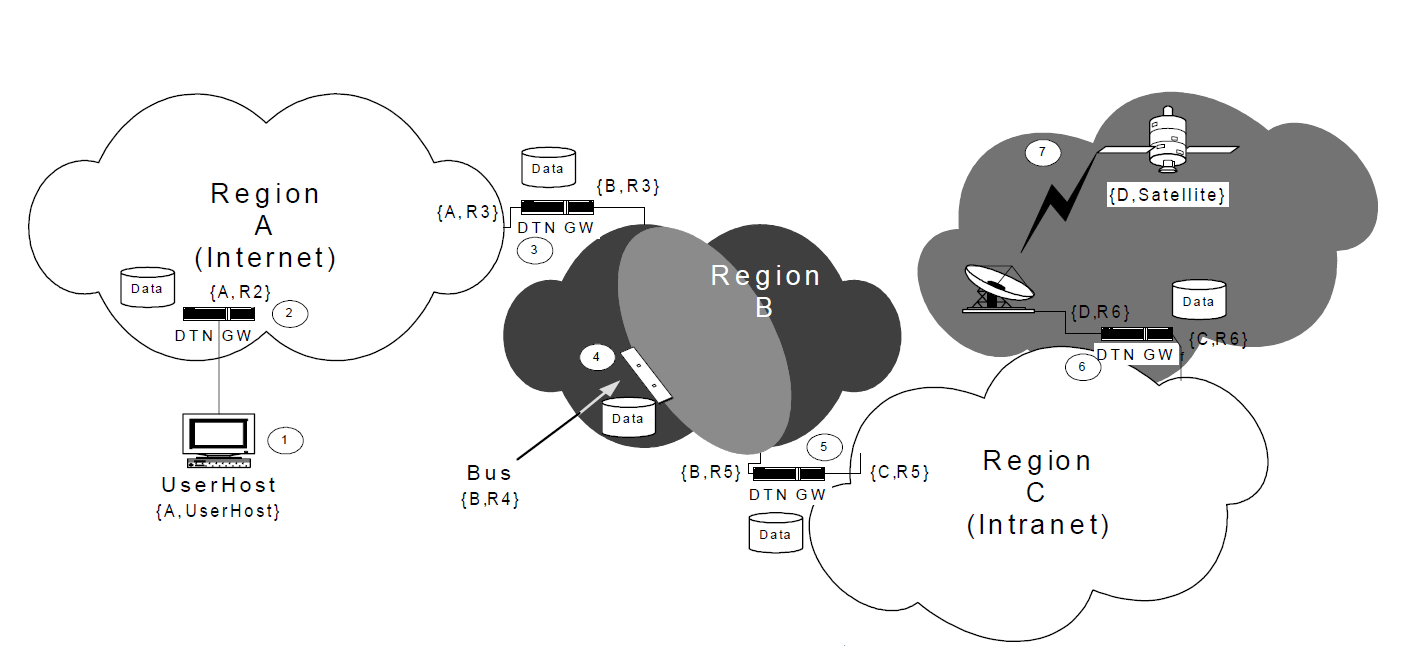
\includegraphics[width=\textwidth,natwidth=1420,natheight=672]{figures/dtn.png}
\caption{Overview of a Delay-Tolerant Network, cited from \cite{Kevin}}
\label{fig:dtn}
\end{figure}

It separates different challenged networks into ``regions" - within each region, nodes communicate under a same protocol, while different regions may run different protocols. As shown in the figure, region A uses Internet, region B uses a bus to deliver messages, region C uses its own Intranet and region C uses satellite to communicate. Different regions are connection by DTN gateways where messages from one region will be routed and forwarded to another region.

One of the key concept of DTN is custody transferring, which refers to the delivery of message from one DTN hop to another together with its reliable delivery responsibility - it's very much like delivering packages through a postal service. And using message couriers to achieve such custody transfer has been accepted as one practical implementation to overcome the difficulties in DTN \cite{Jain}\cite{Zhao}. Although the security issues of DTN have been discussed and evaluated in the high level design of the architecture \cite{Cerf}\cite{Scottrfc} (mainly to maintain efficient routing and prevent abuse of DTN), many security concerns still remain to be considered in the specific courier-dependent message delivery scenario (like what if the courier could be hijacked and examined?). Referencing the high level security framework pre-defined in the architecture, this project will dive into the detail of courier-dependent message delivery and create a practical and efficient security protocol for such scenario.

\subsection{Deniable Authentication}
Privacy protection has been taken much attention to since the communication through digital networks grows dramatically. Most network protocols require authentication as one of its essential steps to achieve secure communication. However, common authentications do not take privacy as one of its goals, thus they require revealing unique identifier of an entity to prove its identity to others - such like a digital signature or a piece of plaintext whose ciphertext can only be decrypted by the entity. As a matter of fact, it is this authentication mechanism disclose the identity of authenticator to third parties. Conversely, in many cases entities want to authenticate themselves to the target entities without revealing their identities to any third parties. This issues have been investigated and analysed by Abadi, who consequently introduced ``private authentication" and presented protocols meet the requirements \cite{Abadi}.

The concept of deniable authentication is created even earlier, by Dwork and Sahai \cite{Dwork}. It indicates the situation that an entity wishes to authenticate a message to the target entity while no any other entities can verify the authentication. Namely, the target entity can not prove the authenticity of the origin of the message to any other entities even itself is convinced by the authentication, thus the message creator can fully deny the existence of the message. It is extremely powerful in terms of privacy protection as combining with privacy authentication, no any private information will be leaked during the authentication. And its repudiation property is proved useful in applications like voting systems and commercial negotiation systems.

So far, many deniable authentication protocols have been invented, they can be sorted as two main classes - interactive \cite{Borisov} and non-interactive \cite{Xin}\cite{Wang}\cite{Shao}. Interactive deniable authentication requires at least 2 messages exchanged during the protocol, one forward and one reply. While non-interactive deniable authentication can achieve the goal in just one message with the cost of heavier computation.

This feature is added in the CDSP to provide an extra level of security to the message being exchanged in order to against potential malicious operations of couriers and message recipients. It might be very important in circumstances like military network or secret message delivery missions.

\section{Motivation and Objectives}
As stated above, this project is inspired by the notion of Delay-Tolerant Network and is specifically designated to create a protocol to improve the security and efficiency for one kind of its custody transferring - courier-dependent communication. More concretely, the invented CDSP should optimize courier-dependent communication in following aspects:
\begin{itemize}
\item Authentication \\
As the cost of such communication will be high - the transportation of courier could be costly, it requires any message delivery request must be authenticated by authorized entity and other entities should be able to check the validity of it.

\item Authenticity of Origin \\
The authenticity of origin of messages should be preserved during the communication, which means when message recipient gets the message, he is able to ensure the message creator. Meanwhile, it implies the integrity of message should be preserved.

\item Confidentiality of Message Content \\
The message content carried by courier should be kept confidential to any entities except the message creator and recipient. Because there is possibility that the courier could be compromised and data it carries may be examined by third parties, courier should gain no knowledge of the actual content it carries.

\item Efficiency \\
Due to the potential limitation of computing and storage capability of Courier and the high cost of such communication, protocol should be designed in such a way that it uses least number of messages and smallest message size to achieve the goal. Especially for cryptography operations, where overhead for encrypting/decrypting messages could be high.

\item Deniability \\
As mentioned above, in secret delivery missions, it would be plausible if Alice is able to deny sending the message in such a way that those who got the message can not prove its authentication to any third parties.
\end{itemize}

\noindent
At the end of the project, following objectives must be achieved:
\begin{enumerate}
\item A fully specified Courier-Dependent Security Protocol should be created and it should meet the requirements mentioned in the above list.
\item A Java library should be developed providing essential functions for implementing the protocol.
\item An application should be built to actually run this protocol.
\item A test of the application should be done to evaluate the performance of the protocol application.
\end{enumerate}

\section{Dissertation Structure}
In the rest of the dissertation, the detailed work will be presented. In Chapter 2 some related works will be discussed, and the differences of this project with those works will be highlighted. Then Chapter 3 will thoroughly describe the system that the protocol serves, including all set-ups, assumptions and rules. It is designated to convey a detailed picture of the scenario. Chapter 4 will fully illustrate the specification of CDSP with the help of message sequencing charts and afterwards, in Chapter 5, the security properties of it will be highlighted and verified. After that, the implementation of the protocol application will be demonstrated in Chapter 6. No concrete code but graphs and charts will be given to give a high level understanding of the work. Then it moves to Chapter 7, where the design of tests and evaluations of the application will be shown and some data will be analysed to show the performance of the protocol. Finally, Chapter 8 will summarise the achievements of the project and draw some reasonable conclusions by pointing out the current system limitation and potential improvements in future work.